\documentclass{article}
  \usepackage{amsmath}
  \usepackage{Sweave}

  %\VignetteIndexEntry{Complete formulas used by coverage}
  %\VignettePackage{actuar}

  \newcommand{\D}{\displaystyle}
  \newcommand{\coverage}{\texttt{coverage}}

  \title{Complete formulas used by \coverage}
  \author{Vincent Goulet}

\begin{document}


\maketitle

The {\coverage} function is used to define a new function to compute
the probability density function (pdf) of cumulative distribution
function (cdf) of any probability law%
\footnote{Provided functions \texttt{pfoo} and \texttt{dfoo} exist in
  the current \textsf{R} frame for probability law \texttt{foo}.} %
under the following insurance coverage modifications: ordinary or
franchise deductible, limit, coinsurance, inflation. In addition, the
function can return the distribution of either the payment per loss or
the payment per payment random variable. For the exact definitions of
these terms as used by {\coverage}, see Chapter~5 of
\cite{LossModels2e}.

In the presence of a deductible, four random variables can be defined:
\begin{enumerate}
\item $Y^P$, the payment per payment with an ordinary deductible;
\item $Y^L$, the payment per loss with an ordinary deductible;
\item $\tilde{Y}^P$, the payment per payment with a franchise
  deductible;
\item $\tilde{Y}^L$, the payment per loss with a franchise deductible.
\end{enumerate}
The most common case in insurance applications is the distribution of
the amount paid per payment with an ordinary deductible, $Y^P$.
Hence, it is the default in {\coverage}.

When there is no deductible, all four random variables are equivalent.

This vignette presents the definitions of the above four random
variables and their corresponding cdf and pdf for a deductible $d$, a
limit $u$, a coinsurance level $\alpha$ and an inflation rate $r$. An
illustrative plot of each cdf and pdf is also included. In these
plots, a dot indicates a probability mass at the given point.

In definitions below, $X$ is the nonnegative random variable of the
losses with cdf $F_X(\cdot)$ and pdf $f_X(\cdot)$.


\section{Payment per payment, ordinary deductible}


\begin{align*}
  Y^P
  &=
  \begin{cases}
    \text{undefined},
      & X < \D \frac{d}{1 + r} \\
    \alpha ((1 + r) X - d),
      & \D\frac{d}{1 + r} \leq X < \frac{u}{1 + r} \\
    \alpha (u - d),
      & \D X \geq \frac{u}{1 + r}
  \end{cases} & \\
  F_{Y^P}(y)
  &=
  \begin{cases}
    0,
      & y = 0 \\
    \D\frac{F_X \left( \frac{y + \alpha d}{\alpha (1 + r)} \right) - F_X
      \left( \frac{d}{1 + r} \right)}{%
      1 - F_X \left( \frac{d}{1 + r} \right)},
      & 0 < y < \alpha (u - d) \\
    1,
      & y \geq \alpha(u - d)
  \end{cases} &
  \begin{minipage}{0.4\linewidth}
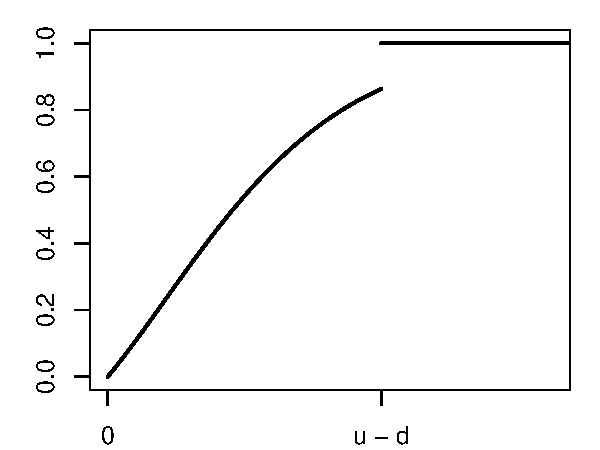
\includegraphics{coverage-004}
  \end{minipage} \\
  f_{Y^P}(y)
  &=
  \begin{cases}
    0,
      & y = 0 \\
    \left( \D\frac{1}{\alpha (1 + r)} \right)
    \D\frac{f_X \left( \frac{y + \alpha d}{\alpha(1 + r)} \right)}{%
      1 - F_X \left( \frac{d}{1 + r} \right)},
      & 0 < y < \alpha (u - d) \\
    \D\frac{1 - F_X \Big( \frac{u}{1 + r} \Big)}{%
      1 - F_X \left( \frac{d}{1 + r} \right)},
      & y = \alpha(u - d)
  \end{cases} &
  \begin{minipage}{0.4\linewidth}
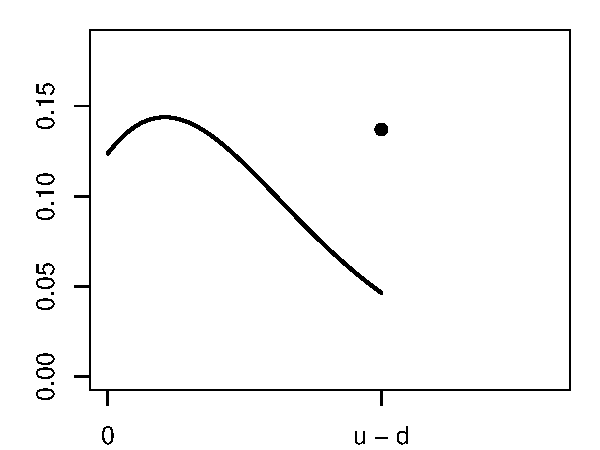
\includegraphics{coverage-005}
  \end{minipage}
\end{align*}


\section{Payment per loss, ordinary deductible}

\begin{align*}
  Y^L
  &=
  \begin{cases}
    0,
      & X < \D \frac{d}{1 + r} \\
    \alpha ((1 + r) X - d),
      & \D\frac{d}{1 + r} \leq X < \frac{u}{1 + r} \\
    \alpha (u - d),
      & \D X \geq \frac{u}{1 + r}
  \end{cases} & \\
  F_{Y^L}(y)
  &=
  \begin{cases}
    F_X \left( \D\frac{d}{1 + r} \right),
      & y = 0 \\
    F_X \left( \D\frac{y + \alpha d}{\alpha(1 + r)} \right),
      & 0 < y < \alpha (u - d) \\
    1,
      & y \geq \alpha(u - d)
  \end{cases} &
  \begin{minipage}{0.4\linewidth}
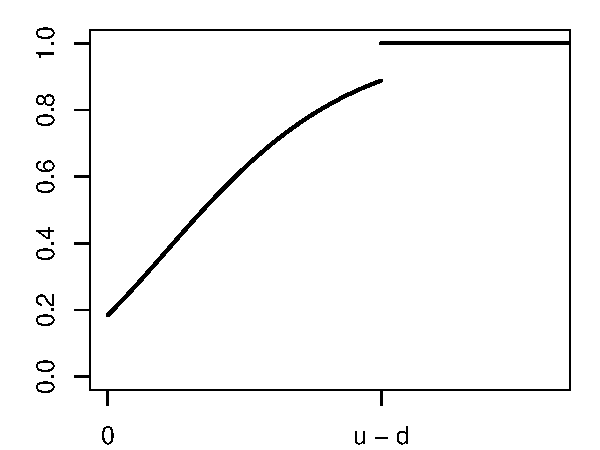
\includegraphics{coverage-006}
  \end{minipage} \\
  f_{Y^L}(y)
  &=
  \begin{cases}
    F_X \left( \D\frac{d}{1 + r} \right),
      & y = 0 \\
    \D\frac{1}{\alpha (1 + r)} f_X \left( \D\frac{y + \alpha
        d}{\alpha(1 + r)} \right),
      & 0 < y < \alpha (u - d) \\
    1 - F_X \left( \D\frac{u}{1 + r} \right),
      & y = \alpha(u - d)
  \end{cases} &
  \begin{minipage}{0.4\linewidth}
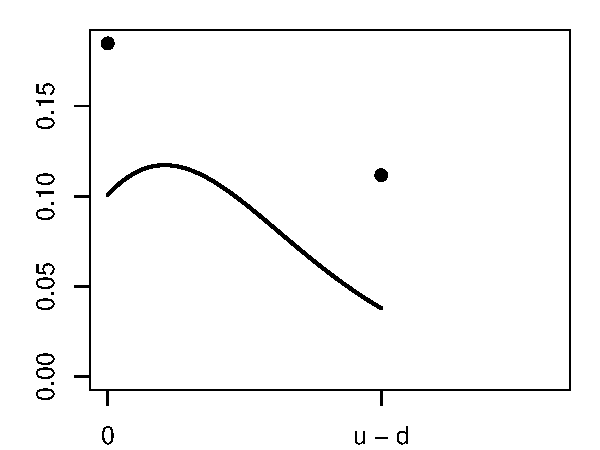
\includegraphics{coverage-007}
  \end{minipage}
\end{align*}


\section{Payment per payment, franchise deductible}


\begin{align*}
  \tilde{Y}^P
  &=
  \begin{cases}
    \text{undefined},
      & X < \D \frac{d}{1 + r} \\
    \alpha (1 + r) X,
      & \D\frac{d}{1 + r} \leq X < \frac{u}{1 + r} \\
    \alpha u,
      & \D X \geq \frac{u}{1 + r}
  \end{cases} & \\
  F_{\tilde{Y}^P}(y)
  &=
  \begin{cases}
    0,
      & 0 \leq y \leq \alpha d \\
    \D\frac{F_X \left( \frac{y}{\alpha (1 + r)} \right) - F_X
      \left( \frac{d}{1 + r} \right)}{%
      1 - F_X \left( \frac{d}{1 + r} \right)},
      & \alpha d < y < \alpha u \\
    1,
      & y \geq \alpha u
  \end{cases} &
  \begin{minipage}{0.4\linewidth}
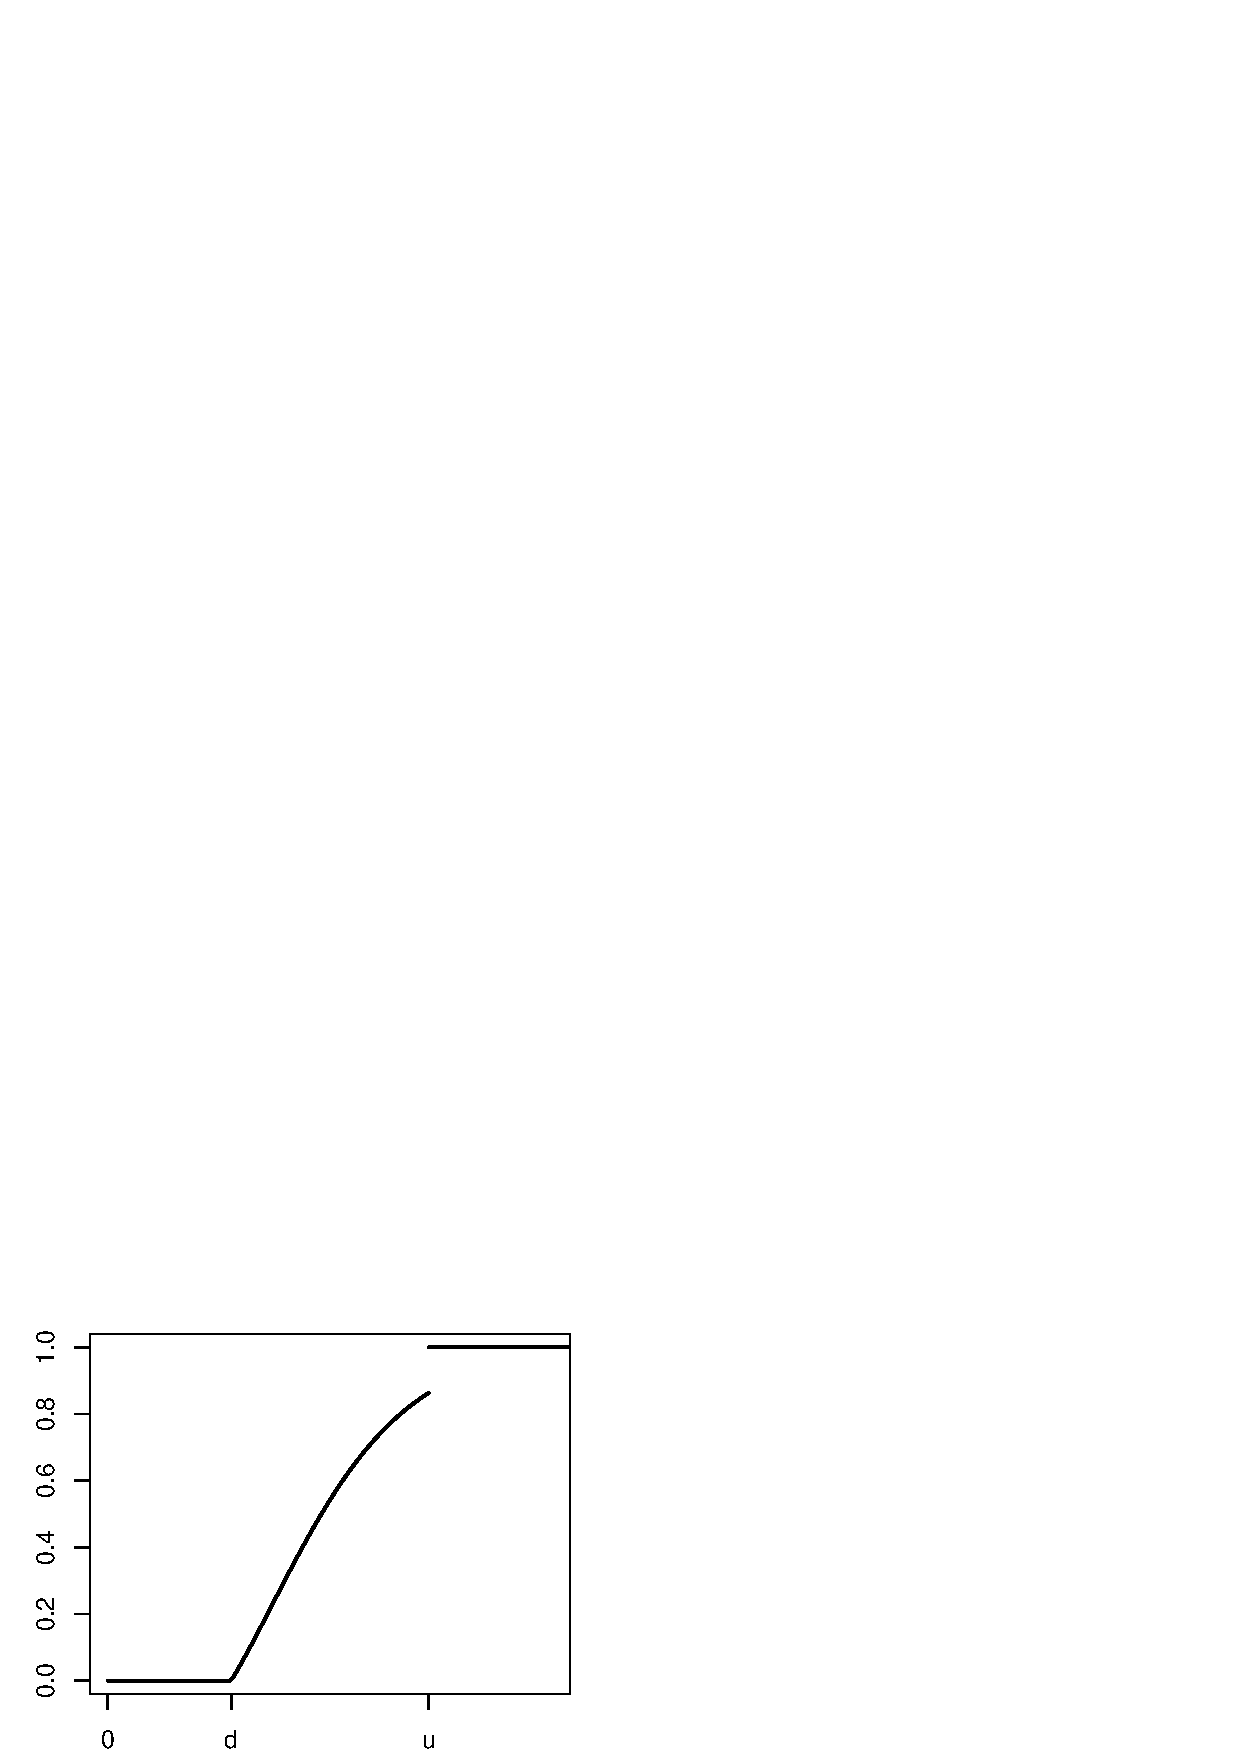
\includegraphics{coverage-009}
  \end{minipage} \\
  f_{\tilde{Y}^P}(y)
  &=
  \begin{cases}
    0,
      & 0 \leq y \leq \alpha d \\
    \left( \D\frac{1}{\alpha (1 + r)} \right)
    \D\frac{f_X \left( \frac{y}{\alpha(1 + r)} \right)}{%
      1 - F_X \left( \frac{d}{1 + r} \right)},
      & \alpha d < y < \alpha u \\
    \D\frac{1 - F_X \Big( \frac{u}{1 + r} \Big)}{%
      1 - F_X \left( \frac{d}{1 + r} \right)},
      & y = \alpha u
  \end{cases} &
  \begin{minipage}{0.4\linewidth}
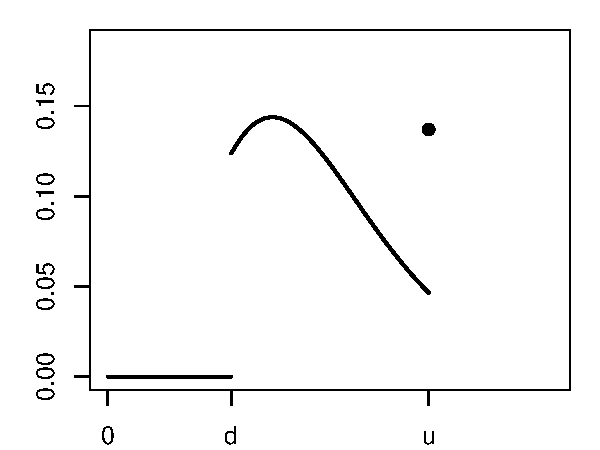
\includegraphics{coverage-010}
  \end{minipage}
\end{align*}


\section{Payment per loss, franchise deductible}

\begin{align*}
  \tilde{Y}^L
  &=
  \begin{cases}
    0,
      & X < \D \frac{d}{1 + r} \\
    \alpha (1 + r) X,
      & \D\frac{d}{1 + r} \leq X < \frac{u}{1 + r} \\
    \alpha u,
      & \D X \geq \frac{u}{1 + r}
  \end{cases} & \\
  F_{\tilde{Y}^L}(y)
  &=
  \begin{cases}
    F_X \left( \D\frac{d}{1 + r} \right),
      & 0 \leq y \leq \alpha d \\
    F_X \left( \D\frac{y}{\alpha(1 + r)} \right),
      & \alpha d < y < \alpha u \\
    1,
      & y \geq \alpha u
  \end{cases} &
  \begin{minipage}{0.4\linewidth}
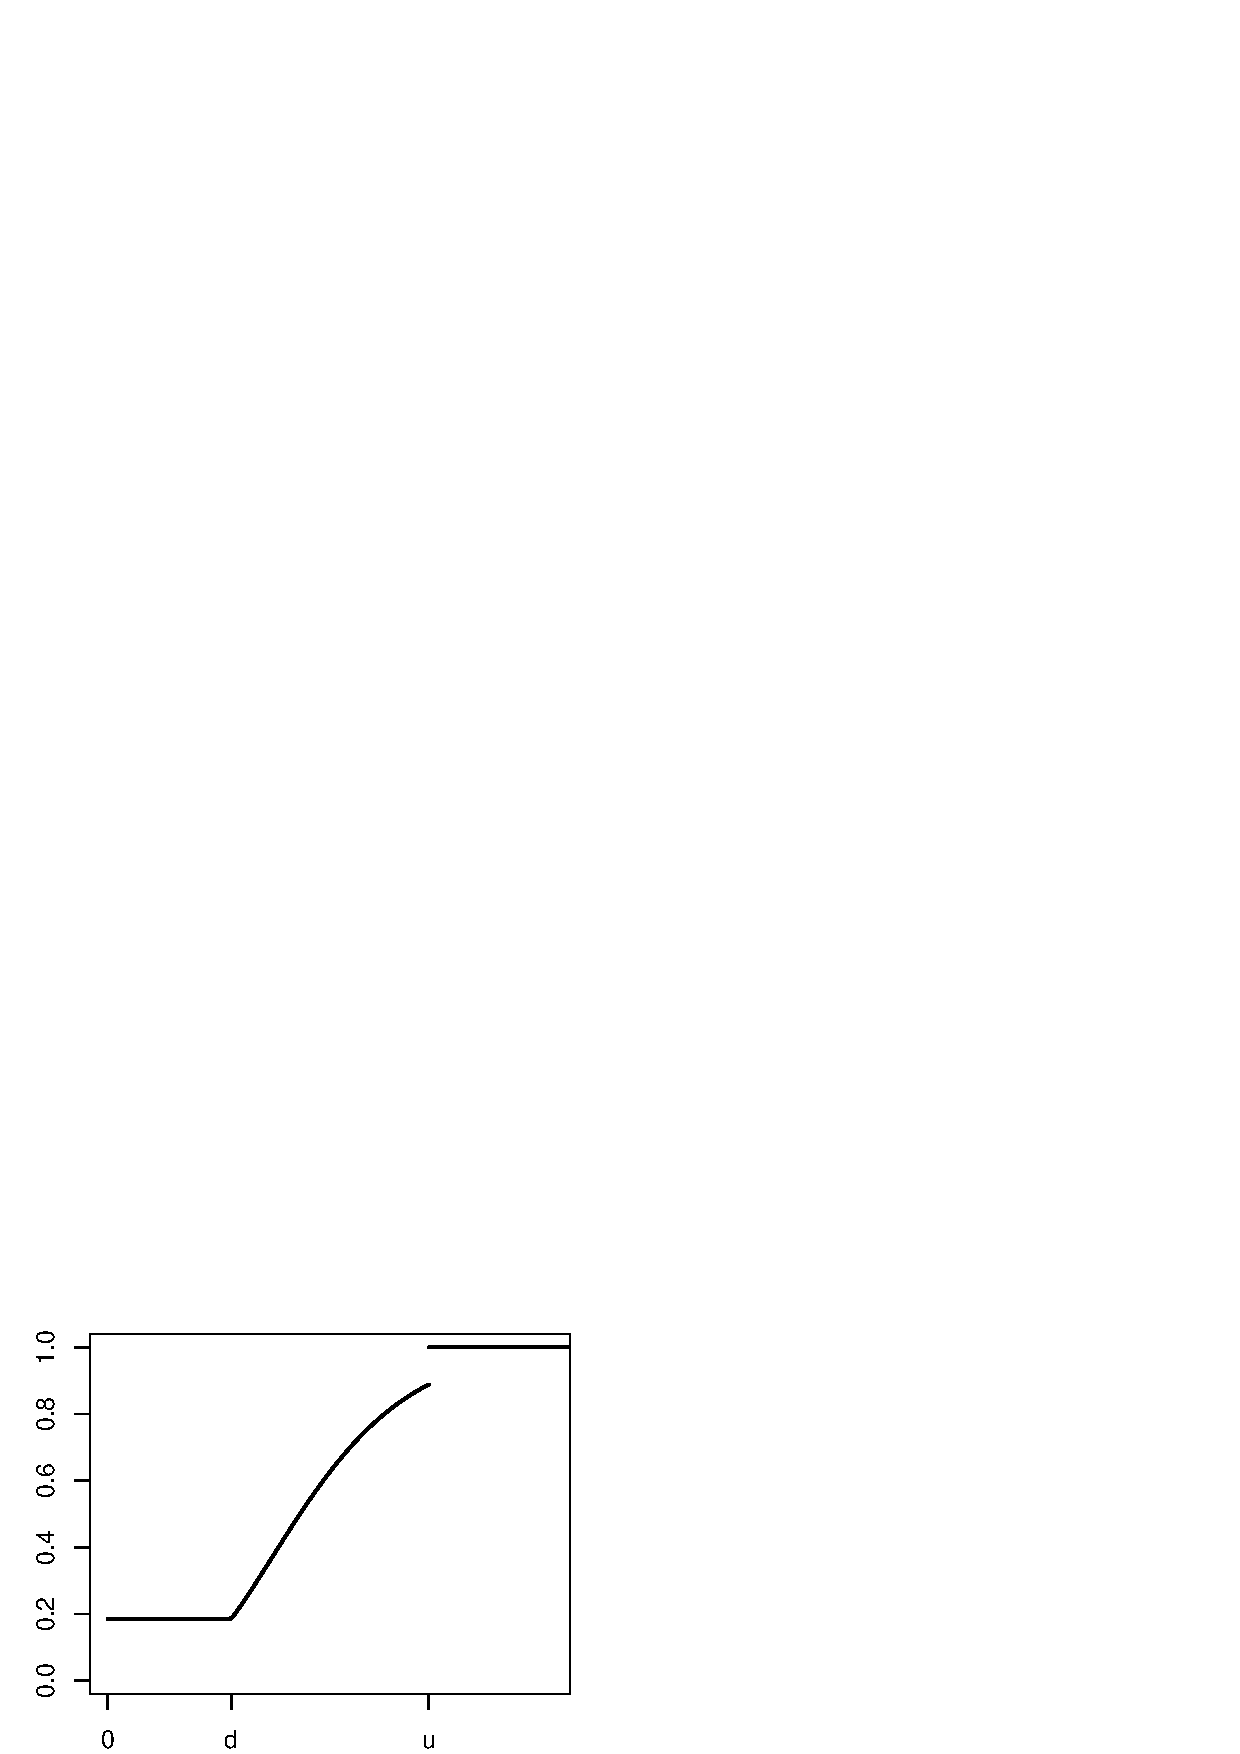
\includegraphics{coverage-011}
  \end{minipage} \\
  f_{\tilde{Y}^L}(y)
  &=
  \begin{cases}
    F_X \left( \D\frac{d}{1 + r} \right),
      & y = 0 \\
    \D\frac{1}{\alpha (1 + r)} f_X \left( \D\frac{y}{\alpha(1 + r)} \right),
      & \alpha d < y < \alpha u \\
    1 - F_X \left( \D\frac{u}{1 + r} \right),
      & y = \alpha u
  \end{cases} &
  \begin{minipage}{0.4\linewidth}
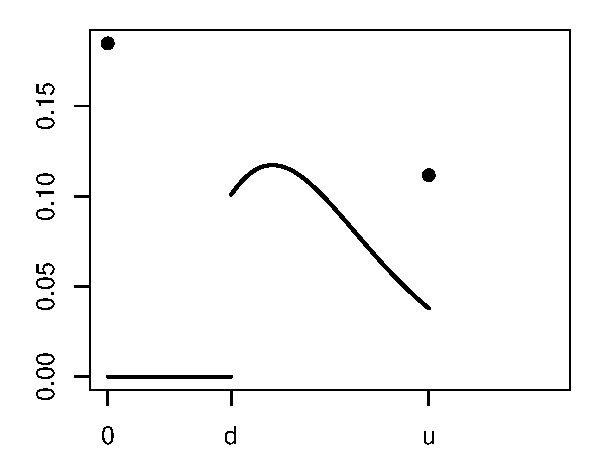
\includegraphics{coverage-012}
  \end{minipage}
\end{align*}

\bibliographystyle{plain}
\bibliography{actuar}

\end{document}

%%% Local Variables:
%%% mode: latex
%%% TeX-master: t
%%% End:
